\chapter{Sicurezza nei sistemi operativi}
Dal manuale sulla sicurezza informatica del NIST (National Institute of Standards and Technology) la sicurezza è la protezione offerta da un sistema informatico automatico al fine di conservare integrità, disponibilità e confidenzialità delle risorse del sistema stesso.

Gli obiettivi che costituiscono il cuore dalla sicurezza sono:
\begin{itemize}
    \item \textit{Integrità}: riferita tipicamente ai dati, che non devono essere modificati senza le dovute autorizzazioni;
    \item \textit{Confidenzialità}: riferita tipicamente ai dati, che non devono essere letti senza le dovute autorizzazioni;
    \item \textit{Disponibilità}: riferita tipicamente ai servizi, che devono essere disponibili senza interruzioni;
    \item \textit{Autenticità}: riferita tipicamente agli utenti, che devono essere chi dichiarano di essere.
\end{itemize}

L'RFC 2828 descrive quattro conseguenze delle minacce informatiche:
\begin{itemize}
    \item Accesso non autorizzato (\textit{Unauthorized disclosure}) quando un'entità ottiene l'accesso a dati per i quali non ha autorizzazione;
    \item Imbroglio (\textit{Deception}) quando un'entità autorizzata riceve dati falsi e pensa siano veri;
    \item Interruzione (\textit{Disruption}) quando si ha l'impedimento al corretto funzionamento dei servizi;
    \item Usurpazione (\textit{Usurpation}) quando il sistema viene direttamente controllato da chi non ne ha l'autorizzazione.
\end{itemize}

Le risorse (o assets) da proteggere sono: hardware, software, dati, linee di comunicazione e reti.

\section{Autenticazione}
Dal punto di vista del sistema operativo un primo passo per garantire meno minacce è l'utilizzo di autenticazione. L'autenticazione si basa su due passi: identificazione e verifica. Determina se un utente è abilitato ad accedere al sistema e i privilegi dell'utente abilitato. Rende possibile il discretionary control access (controllo di
accesso discrezionale) ovvero un utente può decidere a quali utenti concedere determinati
permessi.

L'autenticazione può essere effettuata in diversi modi:
\begin{itemize}
    \item con \textit{password}, è il sistema più noto e usato, ed è importante che le password siano memorizzate non in chiaro.
    \item con \textit{token} che rappresentano oggetti fisici posseduti da un utente per l'autenticazione come memory card o smartcard.
    \item con \textit{biometrica} come impronta digitale, riconoscimento vocale...
\end{itemize}

\section{Controlli di accesso}
I controlli di accesso possono essere:
\begin{itemize}
    \item \textit{Discrezionale} quando un utente può concedere i suoi stessi privilegi ad altri utenti (vedi Figura \ref{fig:controllo-accesso});
    \item \textit{Obbligatorio} quando un utente non può concedere i suoi stessi privilegi ad altri utenti;
    \item \textit{Basato su ruoli} dove ciascun ruolo deve contenere il minimo insieme di diritti d'accesso per il ruolo stesso e un utente viene assegnato ad un ruolo, che lo abilita ad effettuare le operazioni richieste per quel ruolo (vedi Figura \ref{fig:accesso-ruoli}).
\end{itemize}

\begin{figure}[h]
    \centering
    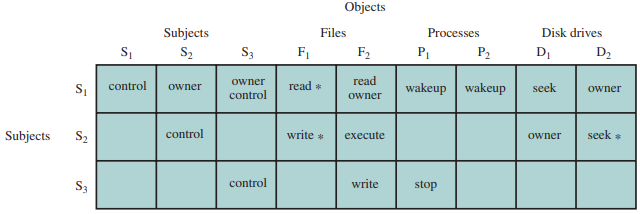
\includegraphics[width=0.7\linewidth]{images/controllo-accesso.PNG}
    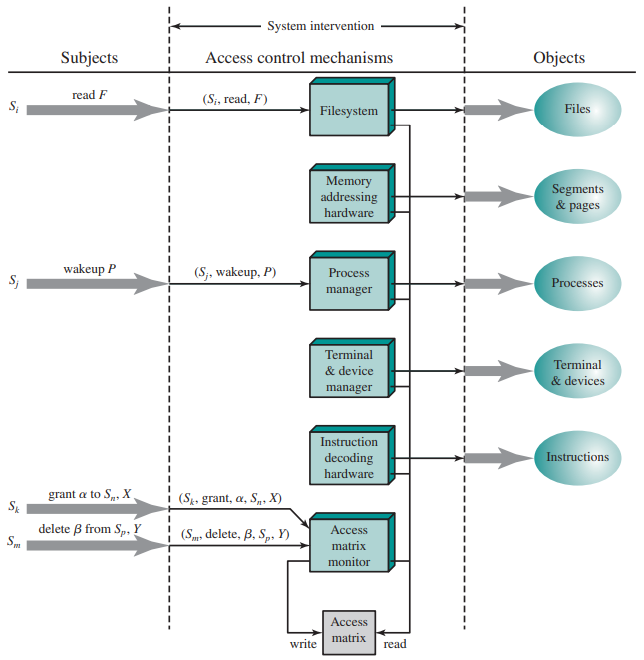
\includegraphics[width=0.6\linewidth]{images/controllo-accesso1.PNG}
    \caption{Controllo di accesso discrezionale}
    \label{fig:controllo-accesso}
\end{figure}

\begin{figure}[h]
    \centering
    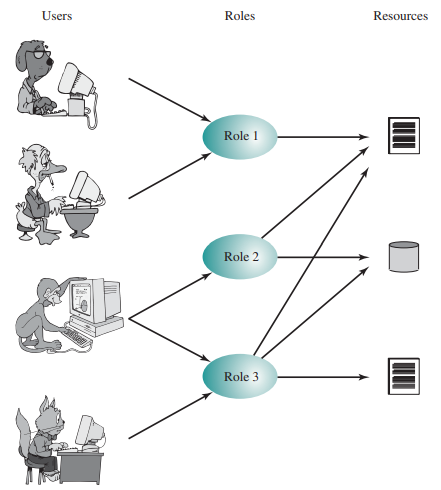
\includegraphics[width=0.5\linewidth]{images/accesso-ruoli.PNG}
    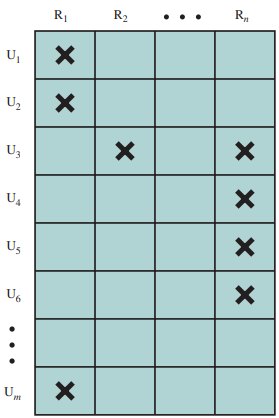
\includegraphics[width=0.3\linewidth]{images/accesso-ruoli1.PNG}
    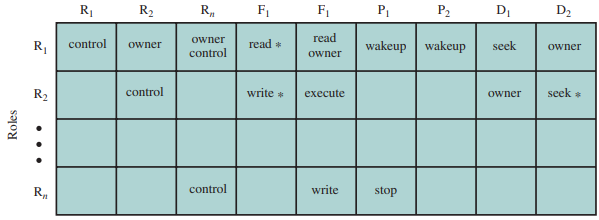
\includegraphics[width=0.8\linewidth]{images/accesso-ruoli2.PNG}
    \caption{Controllo di accesso basato su ruoli}
    \label{fig:accesso-ruoli}
\end{figure}

\section{Protezione in UNIX}
In UNIX la sicurezza è basata sull'autenticazione dell'utente (User-Oriented Access Control) e sui diritti o permessi di accesso ai dati (Data-Oriented Access Control).

Per ogni utente c'è uno username (alfanumerico) e un uid (numerico intero). Lo \textit{uid} è usato ogni volta che occorre dare un proprietario ad una risorsa e ogni utente appartiene ad un gruppo, analogamente identificato da \textit{groupname} e \textit{gid}. Ci sono infine i file di sistema chiamati \verb|/etc/group| e \verb|/etc/passwd| che contengono le informazioni su utenti e gruppi.

Il login può essere fatto su un terminale della macchina (processo \verb|getty|) o tramite rete (\verb|telnet|, \verb|ssh|) e richiede una coppia username e password. Se questa corrisponde ad una entry di \verb|/etc/passwd|, viene eseguita la shell indicata, a partire dalla directory di home indicata. Quando la shell esegue \verb|exit|, o si ritorna al \verb|getty| o si chiude la connessione di rete.

Per ogni file ci sono tre terne di permessi: lettura, scrittura, esecuzione. La prima terna è per il proprietario del file, la seconda per il gruppo cui il proprietario del file appartiene, la terza per tutti gli altri utenti. Le terne di diritti sono usate ogni volta che un processo richiede l'accesso ad un file e se proprietario del file e del processo coincidono, si guarda la prima terna, altrimenti la seconda terna se almeno appartengono allo stesso gruppo, altrimenti la terza terna. Si prende poi l'elemento della terna corrispondente all'accesso richiesto.

\section{Password}
Una password è una stringa di caratteri utilizzata per confermare l'identità di un utente e consentirgli di accedere ad un dispositivo o un servizio.

\subsection*{Password in Linux}
Linux usa due file per gestire utenti e le relative password chiamati \verb|\etc\passwd| e \verb|\etc\shadow|. Entrambi sono normali file di testo con una sintassi similare, ma hanno funzioni e permessi diversi infatti per ogni riga (utente) in \verb|passwd|, esiste una corrispondente riga in \verb|shadow| che indica la sua password.

\verb|\etc\passwd| è un plaintext file, contenente l'intera lista di utenti (account) presenti nel sistema che include non solo utenti “normali”, ma anche utenti standard di sistema e utenti speciali. Ciascuna riga del file \verb|passwd| indica informazioni fondamentali su un utente del sistema, ed ha il seguente fomato:
\begin{itemize}
    \item \textit{Username}: nome dell'utente usato per il login. Stringa alfanumerica di max 32 caratteri;
    \item \textit{Password}: inutilizzato oggi. Il carattere "x" indica che l'hash della password è nel file shadow;
    \item \textit{User ID} (uid): ogni utente nel sistema ha uno user id numerico assegnato;
    \item \textit{Group ID} (gid): una volta creato ogni utente è assegnato ad un primary group (gruppo primario);
    \item \textit{GECOS}: campo descrittivo che contiene informazioni generali sull'utente;
    \item \textit{home directory}: path assoluto alla home directory dell'utente;
    \item \textit{shell}: path assoluto alla command shell usata dall'utente (eseguibile).
\end{itemize}

\verb|\etc\shadow| è un plaintext file contenente, per ciascun utente del sistema, l'hash della sua password ed altre informazioni aggiuntive. Data la criticià delle informazioni contenute, sottrarre e decifrare lo shadow file spesso è uno degli obiettivi principali di un attaccante, conseguentemente ha permessi molto più restrittivi di passwd. Ciascuna riga del file shadow contiene informazioni sulla password del rispettivo utente:
\begin{itemize}
    \item \textit{Username}: nome dell'utente a cui la password appartiene, definito in passwd;
    \item \textit{Password}: password dell'utente salvata usando il Modular Crypt Format;
    \item \textit{Last changed}: data dell'ultimo cambiamento della password, espresso in giorni trascorsi da Unix Epoch (01/01/1970);
    \item \textit{Min Age}: minimo numero di giorni dall'ultimo cambio prima che la password possa essere nuovamente cambiata;
    \item \textit{Max Age}: massimo numero di giorni dopo dei quali è necessario cambiare la password;
    \item \textit{Warn}: quanti giorni prima della scadenza della password va avvisato l'utente.
\end{itemize}

Il \textit{Modular Crypt Format} è il formato usato nello shadow file per salvare gli hash delle password solitamente nel formato \verb|$ID$salt$hash|. L'ID è l'algoritmo di hashing usato per questa password (MD5, blowfish, SHA256, ...); il salt è usato nel processo di hashing; l'hash della password è calcolato con l'algoritmo ID e salt.

La \textit{hash functions} trasforma input di lunghezza variable in output di lunghezza fissa in maniera deterministica (data la stessa stringa in input, darà sempre lo stesso output). Inoltre, una funzione hash è detta crittografica se:
\begin{itemize}
    \item E' computazionalmente difficile calcolare l'inverso della funzione hash;
    \item E' computazionalmente difficile, dato un input $x$ ed il suo hash $d$, trovare un altro input $x_1$ che abbia lo stesso hash $d$;
    \item E' computazionalmente difficile trovare due input diversi di lunghezza arbitraria $x_1$ e $x_2$ che abbiano lo stesso hash $d$.
\end{itemize}

\subsection*{Attacchi a password}
Ma perché non cifrare direttamente la password? In entrambi i casi, le password non sono leggibili da un attaccante: se si usa cifratura ed un attaccante ottiene la chiave, potrebbe decifrare ed ottenere tutte le password in plaintext; le funzioni hash sono one-way ovvero una volta fatto l'hash, non si torna più indietro; se un attaccante ottiene l'hash, non potrà mai scoprire la password che l'ha generato (a parte eccezioni, vedremo poi); è comunque semplice verificare se una password corrisponde a quella salvata in formato hash infatti basta fare l'hash della password
e verificarne l'equivalenza (hashing è deterministico). Questo non vuol dire che gli hash di password siano inattaccabili, esistono due tipi di attacchi: attacco dizionario e attacco Rainbow Table.

Per l'\textit{attacco dizionario} il problema nasce quando ci sono un numero infinito di password che possono
risultare nello stesso hash ma gli utenti sono pigri e non vogliono (o non possono) ricordarsi password molto complesse e non vogliono ricordarsi molte password. Di conseguenza vengono utilizzate password brevi e semplici e riusate molte volte. E possibile dunque compilare una lista di password comunemente utilizzate e fare bruteforce. Un attacco dizionario è molto semplice da effettuare (richiede solo una lista di password), è versatile perché funziona per qualsiasi funzione hash... e ci sono moltissimi tool disponibili per automatizzare il tutto. D'altro canto può essere molto lento, in quanto richiede la computazione in real time degli hash e la password può non essere presente nel dizionario.

Con l'\textit{attacco Rainbow Table} le funzioni hash sono deterministiche in quanto data una lista di password ed una funzione hash, l'hash computato sarà sempre lo stesso per ciascuna password. Una Rainbow Table è un dizionario di coppie (valore hash, plaintext password) creato offline e usato per trovare velocemente quale password corrisponde ad un hash. Un attacco Rainbow Table è molto semplice da effettuare, data la rainbow table precompilata ed è molto più veloce rispetto a dictionary bruteforce. Però una Rainbow Table funziona solo per la funzione di hash per la quale è stata creata la rainbow table, se si vogliamo più funzioni, servono più rainbow tables.

Come fare per proteggersi da questi attacchi? Il salt è un valore randomico, generato quando un utente sceglie la password, che viene aggiunto alla computazione dell'hash. Il salt viene poi salvato in chiaro assieme all'hash calcolato e rende impossibile l'uso di rainbow tables se per ogni utente c'è un salt randomico diverso e se due utenti con la stessa identica password avranno due hash diversi, perché molto probabilmente i loro salt saranno diversi.

\section{Buffer overflow}
L'area di memoria di un processo caricato in memoria è diviso in stack, heap, data e text.

Lo stack è costituito da stack frames, dove ciascun frame contiene dei parametri passati alla funzione, variabili locali, indirizzo di ritorno, instruction pointer. Lo stack pointer punta alla cima dello stack (indirizzo più
basso) e il frame pointer punta alla base del frame corrente. Vengono aggiunti/salvati sullo stack: i parametri passati alla funzione; l'indirizzo di ritorno; il puntatore allo stack frame; spazio ulteriore per le variabili locali della funzione chiamata (vedi Figura \ref{fig:stack-funzione}).

\begin{figure}[h]
    \centering
    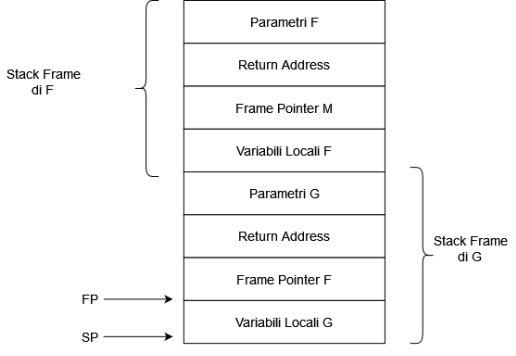
\includegraphics[width=0.5\linewidth]{images/stack-funzione.PNG}
    \caption{Stack di una chiamata a funzione}
    \label{fig:stack-funzione}
\end{figure}

Ipotizziamo di avere il seguente codice:
\begin{lstlisting}[language=C]
    void foo(char *s) {
        char buf[10];
        strcpy(buf, s);
        printf("buf_is_%s\n", s);
    }
    foo("stringatroppolungaperbuf");
\end{lstlisting}

Stiamo inserendo troppi dati rispetto alla dimensione del buffer, il computer non sa la dimensione di buffer, per lui sono solo indirizzi di memoria... Quindi continua a copiare “stringatroppolunga” a partire da primo indirizzo di memoria di \verb|buf[]|, fino a che non ha occupato tutti gli indirizzi di memoria del buffer e poi continua a sovrascrivere qualsiasi cosa trovi, finché non completa l'operazione richiesta.

Di solito, fare overflow di un buffer in questo modo porta alla terminazione del programma. Tuttavia, se i dati che sono usati nell'overflow del buffer sono preparati in modo accurato, è possibile eseguire codice arbitrario. Modificare l'indirizzo di ritorno arbitrariamente è utile, ma come eseguiamo codice arbitrario? Ci sono principalmemte quattro modi per farlo: 
\begin{enumerate}
    \item \textit{Shellcode}. E' un piccolo pezzo di codice che viene eseguito quando si sfrutta una vulnerabilità per attaccare un sistema. E' chiamato shellcode, perché solitamente avvia una command shell, dalla quale l'attaccante può prendere il controllo della macchina. L'idea è inserire codice eseguibile arbitrario nel buffer, e cambiare il return address con l'indirizzo del buffer.

    \item \textit{Return-to-libc}. Non sempre è possibile inserire schellcode arbitrario, tuttavia, esiste del codice utile ad attacchi, che è sempre presente in RAM ed è sempre raggiungibile dal nostro processo. Invece di usare shellcode, possiamo quindi usare come indirizzo di ritorno l'indirizzo di una funzione di sistema utile per un attacco. L'attacco chiamato return-to-libc perché modifica l'indirizzo di ritorno solitamente con l'indirizzo di una funzione standard della libreria C.
\end{enumerate}

Esistono due tipi di contromisure: difese a tempo di compilazione e difese a tempo di esecuzione.

Nel primo caso si possono usare linguaggi di programmazione e di funzioni sicure (l'overflow è possibile perché in C ci sono alcune funzioni che spostano dati senza limiti di dimensione) o con Stack Smashing Protection, dove il compilatore inserisce del codice per generare un valore casuale (canary) a runtime; il valore canary viene inserito tra il frame pointer e l'indirizzo di ritorno; se il valore canary viene modificato prima che la funzione ritorni, interrompi l'esecuzione perché è stato sovrascritto da un possibile attacco.

Nel secondo caso si possono usare Executable Space Protection, dove se un attaccante cerca di eseguire del codice nello stack (shellcode), il sistema terminerà il processo con un errore, oppure Address Space Layout Randomization dove, ad ogni esecuzione, si randomizzano gli indirizzi dove sono caricati i diversi segmenti del programma in modo che se l'attaccante non sa dove inizia lo stack, è molto più difficile indovinare l’indirizzo del buffer contenente lo shellcode.